\documentclass[17pt]{extarticle}
\usepackage{amsmath, amssymb}
\usepackage{nccmath}
\usepackage[a4paper, total={8in, 11.38in},top=2mm,left=27mm,bottom=2mm,right=2mm]{geometry}

\usepackage{tikz}
\usepackage{circuitikz}
\ctikzset{v/.append style={/tikz/american voltages}}

\usepackage{titlesec}
\titleformat{\section}
{\normalfont\normalsize\bfseries}{\thesection}{1em}{}

\titleformat{\subsection}
{\normalfont\normalsize\bfseries}{\thesection}{1em}{}

\begin{document}

\noindent
\begin{fleqn} 

%%%%%%%%%%%%%%%%%%%%%%%%%%%%%%%%%%%%%%%%%%%%%%%%%%%%%%%%%%%%%%%%

\section{Question}
Let  'x'  be the side of a square base and 'h' be the height of the box.\
$\therefore$ Total surface area = $x^2+4h = 300\,cm^2$

\begin{equation} \nonumber
\begin{alignedat}{4}
& \therefore h = \frac{300 - x^2}{4x}\\
& \text{ Base Volume V} \\
&= \text{Area of Base x Height}\\
&= x^2\left(\frac{300-x^2}{4x}\right)\\
&= \frac{1}{4}(300x - x^2)\\
\end{alignedat}
%\vrule
%\vspace{1cm}
\quad\quad\quad
\begin{alignedat}{4}
\begin{circuitikz}[scale=1.5]
\draw (0,0) to [battery1] (0,2) to[short,-o]node[below]{\quad \ \ S$_1$}(0.75,2);
\draw (0.75,2)-- +(30:0.49);
\draw (1.25,2)to[short,o-](2,2);


\draw (2,2) -- (2,2.5);
\draw (2,2) -- (2,1.5);

\draw (2,1.5) to[short,-o] node[below]{\quad \ \ S$_2$}(3,1.5);
\draw (3,1.5)-- +(30:0.49);
\draw (3.5,1.5)to[short,o-] (4.5,1.5);

\draw (2,2.5) to[short,-o]node[below]{\quad \ \ S$_3$}(3,2.5);
\draw (3,2.5)-- +(30:0.49);
\draw (3.50,2.5)to[short,o-](4.5,2.5);

\draw (4.5,2)--(5,2);
\draw (5,2)--(5,1.3);

\draw (4.5,2.5) -- (4.5,1.5);
\draw (5,1) circle(3mm);
\draw (5,1) node{L};


\draw (0,0)--(5,0);
\draw (5,0)--(5,0.7);

\end{circuitikz}
\end{alignedat}
\end{equation}
\quad
\vspace*{-5mm}

%----------------------------------------

\subsection*{Answer}
Let  'x'  be the side of a square base and 'h' be the height of the box.\
$\therefore$ Total surface area = $x^2+4h = 300\,cm^2$



%%%%%%%%%%%%%%%%%%%%%%%%%%%%%%%%%%%%%%%%%%%%%%%%%%%%%%%%%%%%%%%%

\section{Question}
The slant height of a right circular cone is 3 cm. Find the height of cone, if its volume is the greatest.

%----------------------------------------

\subsection*{Answer}
Let  r  and x  be the base-radius and the height of the cone respectively. Then the volume f(x) of the cone is given by

\begin{equation} \nonumber
\begin{alignedat}{4}
f(x) &= \frac{1}{3}\pi r^2x\\
&= \frac{\pi}{3}(3^2-x^2)x\\
&= \frac{\pi}{3}(9x - x^3)\\
\therefore f'(x) &=  \frac{\pi}{3}(9 - 3x^2)\\
\end{alignedat}
%\vrule
\quad\quad\quad
\begin{alignedat}{4}
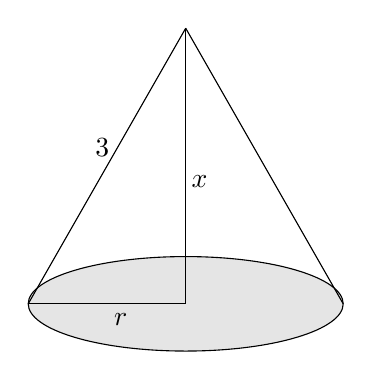
\begin{tikzpicture}
\filldraw[fill=gray!20](0,0) ellipse (2cm and 0.6cm);
\draw (0,0) -- node[below] {\ \ \ $x$}(0,3.5);
\draw (0,0)  -- node[below] {\ \ \ $r$} (-2,0);
\draw  (-2,0) --node[above] {3\ \ }(0,3.5);
\draw  (2,0) -- (0,3.5);
\end{tikzpicture}\\\\
\end{alignedat}
\end{equation}
\begin{equation} \nonumber
\begin{alignedat}{4}
& Now\ f'(x) = 0\ gives\\
& \frac{\pi}{3}(9x - x^3)=0\\
& \therefore \ 3x^2=9\\
& \therefore x = \sqrt{10}
\end{alignedat}
\quad
\vrule
\quad
\begin{alignedat}{4}
& Also\ \ f''(x) =-6x\\
& \therefore\ \ f''(\sqrt{3})=-6\sqrt{3}<0\\
& \therefore \ \ By\ second\ derivative\ test\\
& Volume \ f\ is maximum\ at\ x=\sqrt{3}
\end{alignedat}
\end{equation}
%%%%%%%%%%%%%%%%%%%%%%%%%%%%%%%%%%%%%%%%%%%%%%%%%%%%%%%%%%%%%%%%


\end{fleqn}
\end{document} 